\section{Machine Learning and Deployment \label{deployment_section}}
\acrshort{ml} application has developed from being in domain of academic research to an applied field. A survey conducted by McKinsey \& Company \cite{analytics2019global} shows that nearly 25\% of business processes are adopting machine learning techniques. However, there is a huge difference and challenges to put ML in real world system as compared to academic settings. Reports from Algorithmia \cite{wiggers2019algorithmia, hecht2019add} shows that it takes 8 to 90 days for the majority of companies to deploy a single model and 18\% of companies took even more time to deploy. According to \acrfull{idc}'s report\footnote{\url{https://venturebeat.com/ai/idc-for-1-in-4-companies-half-of-all-ai-projects-fail/},Accessed: 22.03.2024} that includes 2,473 organizations into the survey, A notable portion has failed in an attempt of \acrshort{ai} deployments. Moreover, the \acrshort{idc}'s report points that the reasons could be lack of expertise, bias in data and high costs of resources.

When we talk about deploying ML functionality in production, there are several aspects that should be discuss such as machine learning deployment workflow, ethical considerations, law, end-user's trust, and security which are briefly discussed in \cite{paleyes2022challenges}. The term to make a service or a product using machine learning and making available for users refer as production. Sometimes the term ML deployment workflow also known as ML pipelines and there are various definitions and descriptions of it such as Cros-Industry Standard Process For Data Mining (CRISP-DM) \cite{shearer2000crisp} or Team Data Science Process (TDSP) \cite{TDSP}. In general, the process of developing machine learning based product and services in industrial environment have stages like data management, model learning, model verification and model deployment. Each of these stages can be further broken down in smaller steps as shown in \Cref{tab:deployment_stages} and each steps can run in parallel while informing each other through feedback loops. For developing ML pipelines, one could think of using best practices to use software development principles for productionizing machine learning products and services such as DevOps. It is about fast, flexible and provisioning business processes that integrates development, delivery and operations more efficiently thus pronounce as DevOps. It was an organizational shift from distributed groups or departments that performs function separately to cross-functional teams that works on continuous operational feature deliveries. These principles of DevOps brought a cultural shift towards in the collaboration between areas like development, quality assurance and operations. In paper \cite{ebert2016devops}, authors have presented a comprehensive case study of different tools and micro-services and the impact of these DevOps technologies on industry projects, An overall DevOps model's areas are shown in \Cref{fig:DevOps}. 

\begin{figure}[!ht]
    \centering
    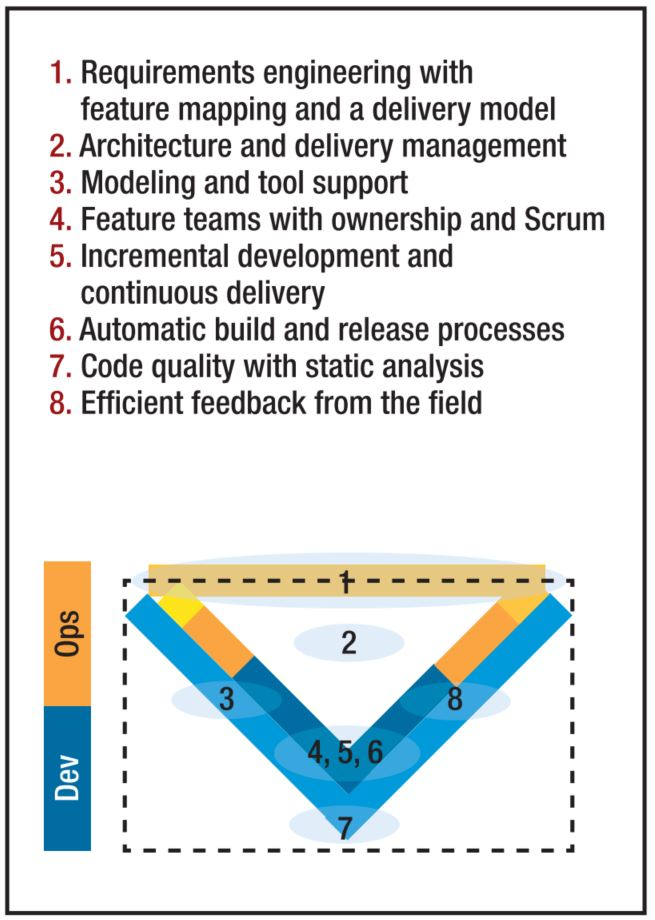
\includegraphics[width=0.45 \textwidth]{chapters/images/Literature_review/DevOps.JPG}
    \caption{A DevOps model infrastructure \cite{ebert2016devops}}
    \label{fig:DevOps}
\end{figure}

Some of these DevOps principles can be directly apply to ML systems but there are number of challenges that are specific to the machine learning, which are briefly discussed in \cite{dang2019aiops}, this paper introduced the term AIOps (also recognized as MLOps) that refer as DevOps tasks for ML systems. The market for machine learning services and tools is already started gaining growth. There are new tools and services being introduced continuously in order to overcome the problems in the deployment process. For example platforms like AWS SageMaker\footnote{\url{https://aws.amazon.com/sagemaker/},Accessed: 22.03.2024}, AzureML\footnote{\url{ https://azure.microsoft.com/en-us/products/machine-learning}, Accessed: 22.03.2024}, TensorFlow TFX\footnote{\url{https://www.tensorflow.org/tfx}, Accessed: 22.03.2024}, MLflow\footnote{\url{https://mlflow.org/}, Accessed: 22.03.2024} and so on helps in various stages of deployment by providing services like data storage, retraining and model hosting with \acrfull{api} for training and inference operations, special set of metrics for monitoring model performance and health and interface for custom changes. These platforms offer managed infrastructures that helps decreasing the burden on the people associated to maintain the operations of ML model in production. Platforms like these allowed people to actively contribute in a communities and build tools and libraries for different aspects in deployment stages. For example, to check quality, CheckList methodology \cite{ribeiro2020beyond} gives formal approach to check the quality of \acrshort{nlp} models, The Data Linter \cite{hynes2017data} to inspect the dataset for potential issues. Tools like Auto-keras\footnote{\url{https://autokeras.com/}, Accessed:03.04.2024}, Auto-sklearn\footnote{\url{https://www.automl.org/automl-for-x/tabular-data/auto-sklearn/}, Accessed: 03.04.2024} aims to provide general-purpose implementations for machine learning algorithms. Though new tools for ML tasks are being released constantly, Practitioner still have to have knowledge of right tool and the dependencies at different deployment stages.




%######################devOps bib name : ebert2016devops


% Please add the following required packages to your document preamble:
% \usepackage{multirow}
% Please add the following required packages to your document preamble:
% \usepackage{multirow}
% Please add the following required packages to your document preamble:
% \usepackage{multirow}
% Please add the following required packages to your document preamble:
% \usepackage{multirow}
\begin{table}[H]
\begin{tabular}{|l|l|l|}
\hline
                  \textbf{Deployment Stage}&\textbf{Deployment Step}& \textbf{Considerations, Issues, and Concerns} \\ \hline
\multirow{7}{*}{Data management} &                   Data collection&  Data discovery\\ \cline{2-3} 
                  & \multirow{2}{*}{Data preprocessing} &  Data dispersion\\  
                  &                                     &  Data cleaning\\ \cline{2-3} 
                  & \multirow{3}{*}{Data augmentation}  &  Labeling of large volumes of data\\ 
                  &                                     &  Access to experts\\ 
                  &                                     &  Lack of high-variance data\\ \cline{2-3} 
                  &                   Data analysis     &  Data profiling\\ \hline
\multirow{9}{*}{Model learning} & \multirow{2}{*}{Model selection}   &  Model complexity\\ 
                  &                                     &  Resource-constrained environments\\ 
                  &                                     &  Interpretability of the model\\ \cline{2-3} 
                  & \multirow{3}{*}{Training}           &  Computational cost\\ 
                  &                                     &  Environmental impact\\ 
                  &                                     &  Privacy-aware training\\ \cline{2-3} 
                  & \multirow{3}{*}{Hyper-parameter selection} &  Resource-heavy techniques\\ 
                  &                                     &  Unknown search space\\ 
                  &                                     &  Hardware-aware optimization\\ \hline
\multirow{6}{*}{Model verification} & \multirow{2}{*}{Requirement encoding} & Performance metrics \\
                  &                                     & Business-driven metrics\\ \cline{2-3} 
                  &                 Formal verification &  Regulatory frameworks\\ \cline{2-3} 
                  & \multirow{3}{*}{Test-based verification} &  Simulation-based testing\\ 
                  &                                     &  Data validation routines\\ 
                  &                                     &  Edge case testing\\ \hline
\multirow{9}{*}{Model deployment} & \multirow{4}{*}{Integration} &  Operational support\\ 
                  &                   &  Reuse of code and models\\ 
                  &                   &  Software engineering anti-patterns\\ 
                  &                   &  Mixed team dynamics\\ \cline{2-3} 
                  & \multirow{3}{*}{Monitoring} & Feedback loops  \\ 
                  &                   &  Outlier detection\\
                  &                   &  Custom design tooling\\ \cline{2-3} 
                  & \multirow{2}{*}{Updating} & Concept drift  \\
                  &                   &  Continuous delivery\\ \hline
\end{tabular}
\caption{Considerations, Issues and Concerns in different deployment stage \cite{paleyes2022challenges}}
\label{tab:deployment_stages}
\end{table}

































\section{Cloud Computing for ML Deployment}

Internet keeps changing the way people work, learn, communicate and so on. It has influenced from one individual to entire industries. Rapid development of processing and storage technologies helped to reduce the cost of computing while increasing power and availability. This technological advancement provided a realization of a computing model called "Cloud Computing". Users can lease and release the resources like CPU and Storage in an on-demand manner. In general, the cloud computing infrastructure can be divided into two prime roles. One, the infrastructure provider responsible to manage cloud platforms. Second, service-provider, who consume these resources from infrastructure-providers and servers different services to end users. Cloud technologies have influenced the Information Technology (IT) industries and Companies like Google, Microsoft and Amazon provides cloud-platforms which help enterprises to develop, reshape their business models and gain benefits such as no up-front investment in resources since now they can just rent the infrastructure as they uses, which is also known as pay-as-you-go pricing model, high scalability, easy access and more important risks and maintenance. Using cloud infrastructure means we are simply outsourcing the risks such as hardware failures to the infrastructure providers who are better equipped to manage these risks that helps to decreasing the cost on maintenance and training of staff. In paper \cite{lee2013view}, Author presents results of an economic view of IBM cloud computing engagements \ref{tab:IT_benifits}.


\begin{table}[hb]
    \centering
    \begin{tabular}{|c|c|c|c|}
    \hline
         & Tasks & Traditional Computing &  Cloud Computing \\
    \hline
    \multirow{6}{5em}{Increasing speed and flexibility} & Test provisioning & Weeks & Minutes \\ 
        & Change Management & Months & Days/hours \\ 
        & Release Management & Weeks & Minutes \\
        & Service Access & Administered & Self-service \\ 
        & Standardization & Complex & Reuse/Share \\
        & Metering/billing & Fixed Cost & Variable Cost \\
    \hline
    \multirow{2}{5em}{Reducing Costs} & Server/storage utilization & 10-20\% & 70-90\% \\
        & Payback period & Years & Months \\
    \hline
    \end{tabular}
    \caption{Benifits of Cloud Computing}
    \label{tab:IT_benifits}
\end{table}



\subsection{Overview of cloud Architecture}

The architecture of cloud computing environment is made of sublayers such as Infrastructure as a service (Iaas),  Platform as a Service (Paas) and Software as a Service (SaaS) as show in \Cref{fig:Layers_of_Cloud_Architecture}. Each layer is coupled with layers above or below in a way that each layer can evolved separately allowing applications to be better at management and maintenance. 

\begin{figure}[!ht]
    \centering
    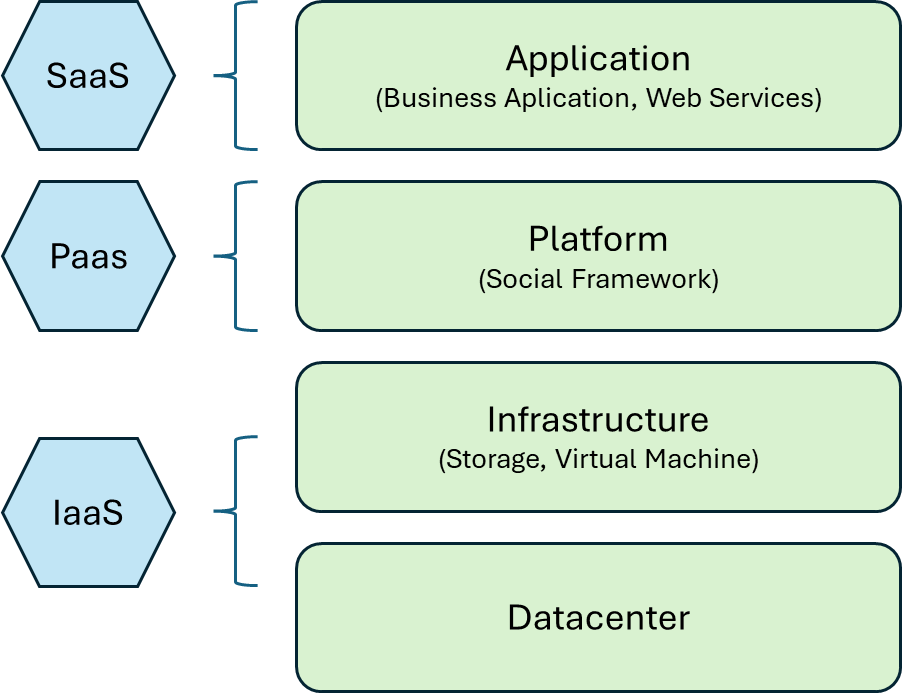
\includegraphics[width=0.5\textwidth]{chapters/images/Cloud_Computing/Cloud_layers.png}
    \caption{Layers of Cloud Architecture}
    \label{fig:Layers_of_Cloud_Architecture}
\end{figure}

\subsubsection{Infrastructure as a Service - IaaS}
The layer IaaS includes resources like data centers that contains servers, routers, power and cooling systems and so on. Therefore, also known as a hardware layer. It also contains the infrastructure layer that includes pool of storage and computing resources like virtualization technologies therefore also known as virtualization layer. IaaS usually refers to providing resources on-demand mostly in forms of Virtual Machines for instance Amazon EC2\footnote{\url{https://aws.amazon.com/pm/ec2/}, Accessed: 06.05.2024}.

\subsubsection{Platform as a Service - PaaS}

This layer is build on top of the infrastructure layer that includes different operating systems and application frameworks. PaaS-provider delivers necessary hardware and software tools over internet for users which allows to focus on deployment and management of their application. 

\subsubsection{Software as a Service - SaaS}

Saas is the layer where the actual cloud application is being served that reaches to end-user and it is at the top of the hierarchy. It is different from ordinary served application in terms of highly-scalable since this layers have automatic-scaling feature to achieve better performance, availability and lower operating cost.

\subsection{Machine Learning and Cloud Computing}

Cloud infrastructure outperforms the traditional way of serving the ML models in terms of performance and cost, many of these cloud provider are focusing on developing new architectures that are specifically developed for workloads like neural networks and deep learning, Implementing features like specialized cores to increase matrix operations for instance Google TPUs (Tensor Processing Units) \cite{google_tpu}. In addition, the elasticity, flexibility and economy is making cloud computing more suitable for deploying machine learning models. The different layer model of cloud makes it easy to deploy various infrastructure components on different layers that helps to manage these resources in efficient ways. Cloud providers offers inbuilt PaaS and SaaS a step ahead from low-level offerings like IaaS to enable large-scale computing infrastructures with easy-to-use services with respect to Machine learning "as-a-Service" for end users. Today's data-centers are located in various part of the world. Using services available in PaaS/ SaaS one can deploy their services or product on distributed infrastructures which is accessible trough internet. 

Cloud computing enabled companies to build their products and collaborate on a global level. For instance Hugging face \cite{huggingfacehub} provides a platform where companies or individuals can build their own AI, leverage open source models and technology and make it easy for data scientist, machine learning engineers and developers to collaborate. Users can easily access these models and applications with the hardware capabilities of Google Cloud \cite{Googlecloud} such as TPU instances, Virtual Machines, NVIDIA H100 Tensor Core GPUs \cite{Nvidiagpu} and so on. Currently, there are approx more than 400 thousand models, 150 thousand application and 100 thousand datasets available on hugging face \cite{huggingfacehub}. Some of them may come with copyrights or Licences to use and assets like  Open-Source, anyone can access to these pre-trained models which are already well trained and architected, one can fine-tune it and use it for their downstream tasks with their own datasets or the available datasets without investing on large resource required to set up IT infrastructure to serve high computing services like machine learning on Hugging face by just using internet through their laptops in a pay-as-you-go manner.


